%% example for producing articles in MVA format using LaTeX.
%% written by Takeshi MASUDA, Electrotechnical Laboratory, Japan in May 1996.
%% modified by KAGESAWA Masataka, OKAZAKI Shin'ichro, YASUMOTO Mamoru.
%% last modified by Masaki Onishi, AIST, in Nov 2012.
%% use at your own risk.

\documentclass{mva_style}
\usepackage{graphicx}
\usepackage{color}
\usepackage[utf8]{inputenc}
\usepackage{xurl}

\finalcopy %Uncomment this line for the Camera-Ready Manuscript

\begin{document}
\title{Sickle Cell Disease | A Review}

\author{
  Samim Khaleqi\\
  HSC Biology\\
  Bellfield College\\
  10.6084/m9.figshare.28701725
}

\maketitle


\section{Introduction}
\subsection{What is a Mutagen?}
A mutation is a change of DNA sequence in an organism; these mutations are caused by an error in DNA replication, exposure to mutagens (naturally occurring and synthetic), and germline mutations (gametes) can increase this rate of mutation. (Gilchrist, 2019)

\subsection{How Mutagens Operate}
Mutations in DNA are caused by mutagens, and these mutagens cause mutagenic effects. These mutagens can be chemicals (benzene, tar in smoke, asbestos, etc.) or forms of radiation (these include ultraviolet (UV) light and ionising radiation). These mutagens can cause irreversible and carcinogenic (cancer-causing) effects (Schrader, 2003).
Chemicals ingested (tar in tobacco smoke, etc.) or environmental irritants (benzene, asbestos, etc.) are mutagenic due to their similar chemical structure to the nucleotide base pairs; this makes them susceptible to the insertion of the wrong nucleotide pair in DNA, which leads to mispairing (Chidrawi et al., 2018).

Additionally, there exist naturally occurring mutagens that can be biological or non-biological. Biological mutagens such as viruses work by injecting their own DNA into the DNA of host cells, potentially changing the function of the cell and triggering cancers. Non-biological occurring mutagens, however, include naturally occurring substances such as mercury and cadmium that can disrupt the cell cycle, leading to faulty DNA replication (Chidrawi et al., 2018) (Shendure and Akey, 2015).

\subsection{Causes of Mutation}

Two types of mutations exist: point mutations, where a single nucleotide is changed in the genetic sequence, and chromosomal mutations, large-scale changes where sections of chromosomes are altered (Chidrawi et al., 2018).  
Point mutations include:
\begin{itemize}
    \item Frameshift: insertion/deletion, where a nucleotide is removed or added; this causes the entire section of nucleotides to shift left or right; this causes major changes as the amino acid sequence is affected; examples include Huntington's disease.
    \item Nonsense mutation: when a codon pair changes into a stop codon, it usually results in non-functional proteins and has a major phenotypic effect.
    \item Missense mutation, where a nucleotide change causes an amino acid to change, this usually leads to a less functional protein; examples include sickle cell, where the haemoglobin has reduced oxygen capacity.
    \item Silent mutation, where a nucleotide change gives the same amino acid in the polypeptide chain, silent mutations thus give no change to the protein and phenotype.
\end{itemize}

Chromosomal mutations include:
\begin{itemize}
    \item Deletion, where a part of a chromosome is removed. This reduces the number of genes in a chromosome.
    \item Duplication, where an extra section of chromosomal DNA is added.
    \item Inversion, where a piece of the chromosome gets removed, rotates \begin{math}180^o\end{math} and is added back to the original chromosome.
    \item Translocation, where two chromosomes split apart and pieces mix up to form heterozygous chromosomal pairs.
\end{itemize}

These mutations are usually caused as a result of DNA breakage due to mutagens such as radiation, chemicals, or errors in meiosis.

\subsection{Somatic and Germline Mutations}
Depending on the cell, two types of mutations can occur: somatic and germline mutations.
Somatic cell mutations are mutations that occur within non-reproductive body cells (examples include skin and liver cells). These mutations are usually caused by environmental factors such as UV radiation or DNA replication errors during S phase in mitosis. If the error goes undetected in the G2 phase, the following mutation will be passed onto its daughter cells; with each division, the mutation gets amplified. It is important to note that even though the mutation passes to daughter cells, it will not pass onto offspring due to it occurring in a non-reproductive cell. This mutation may be expressed in the phenotype, such as skin cancer from UV-damaged skin cells; however, this is not always the case (Chidrawi et al., 2018). Sometimes a somatic mutation can have a physiological effect, such as paroxysmal nocturnal hemoglobinuria (PNH), a somatic frameshift mutation on the PIGA gene leading to the removal of proteins CD55 and CD59; this makes the immune system attack the red blood cells, leading to anaemia (Medline Plus, n.d.).

On the other hand, germ-line (genetic) mutations are mutations that occur within reproductive cells, gametes (germline cells). Mutations that occur within these cells are passed onto offspring, making them hereditary (National Cancer Institute, 2012), unlike somatic cells, which are not. Additionally, germ-line mutations affect every cell in the body due to the mutation fusing with the other gamete during the formation of the embryo, rather than somatic cells only affecting the localised area of mutation (Chidrawi et al., 2018). Examples of germ-line mutations include down syndrome, a duplication of the 21st chromosome (Akhtar and Bokhari, 2023), and sickle cell disease, a point mutation of the 6th codon pair in the beta-globin gene, leading to the distinct ’sickle’-shaped red blood cells (National Heart, Lung, and Blood Institute, 2024). 

\begin{figure}
    \centering
    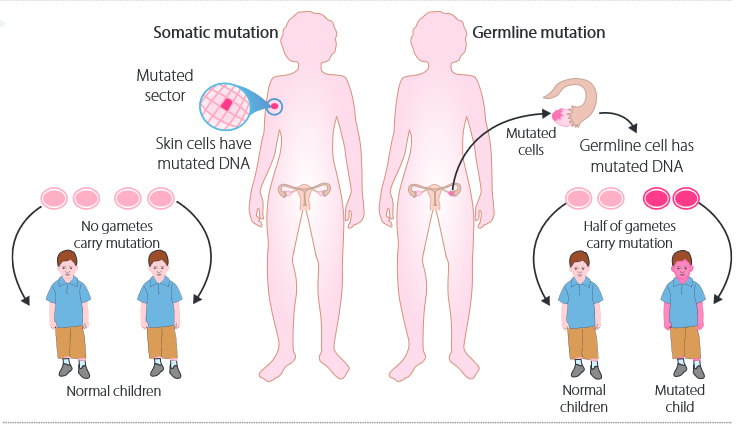
\includegraphics[width=0.8\linewidth]{img/Chidrawi et al., 2018, Figure 7.12.png}
    \caption{Somatic and germline mutations. (Chidrawi et al., 2018, Figure 7.12)}
    \label{fig:enter-label}
\end{figure}

\subsection{Coding and Non-coding DNA significance}
DNA in the human genome is split into two groups: coding DNA, which accounts for 1.5\% of the genome, and non-coding DNA, which accounts for 98.5\% of the genome (Richard Boland, 2017) (Mattick and Amaral, 2022).
Coding DNA regions are used to transcribe mRNA into proteins; therefore, mutations in coding DNA can change the function or levels of a protein (Chidrawi et al., 2018). An example of this is sickle cell disease, where the haemoglobin protein produces a wrong amino acid; this change leads to a less functioning protein (Kato et al., 2018). Additionally, mutations in the DNA repair enzymes can cause other mutations to go unfixed, leading to spontaneous cell function before the cell becomes cancerous or self-destructs (Chidrawi et al., 2018).
Non-coding DNA regions, initially thought to be junk, are quite important to the regulation of DNA. These sequences control which genes should be expressed and which should not; additionally, changes that occur in the microRNA control which introns are removed from the cell before it's used for translation, so such changes in these noncoding regions can have an effect on gene expression and cell function (Chidrawi et al., 2018). An example of this is b-thalassemia, where the beta-globin promoter is affected, reducing the amount of haemoglobin A in red blood cells, leading to anaemia (Needs, Gonzalez-Mosquera, and Lynch, 2023).

\subsection{Mutation Effect on Gene Pool}
A gene pool is the genetic composition of a population; the gene pool (alleles) is affected by three main factors: mutation, gene flow, and genetic drift.
Mutations allow for random changes in DNA sequence to create new alleles; these changes can be either positive or negative, and only changes occurring in germ-line cells are passed on and enter the gene pool (Chidrawi et al., 2018). Examples of gene pool mutations include peppered moths, where a mutation in the M1CR gene increased melanin production, helping them to camouflage in the post-industrial revolution (Majerus and Mundy, 2003). 
Gene flow is the movement of alleles in a population due to the introduction or removal of individuals. This can introduce new alleles or remove them from a population and counteract genetic drift by introducing lost alleles.
Genetic drift refers to the allele frequencies due to random events such as natural disasters, the founder effect, or human activity; these events can be catastrophic to populations as their gene pool can be reduced, leaving them susceptible to disease, though it is much more negligible in large populations (Chidrawi et al., 2018). Examples include northern elephant seals, who have lost 98\% of their gene pool due to mass hunting (Hoelzel et al., 2024).

\subsection{Inquiry Question}
This depth study will be looking at how a mutation in the HBB gene can lead to sickle cell disease and its effects on an individual, including its treatment and prevention.

\section{Cause and Effect}
The human body requires red blood cells (RBCs) for healthy bodily function. RBCs are made up of approximately 200-300 million haemoglobin (Hb) proteins; each haemoglobin protein contains 4 globin polypeptide chains, two beta and two alpha called HbA, with a hydrophilic (water-attracting) exterior and hydrophobic (water-repelling) heme group (Sheffield, 2017). Haemoglobin functions by transporting oxygen from the lungs to tissue and carbon dioxide from the tissue to the lungs to provide for cellular respiration (Schnog et al., 2004).
Two additional haemoglobin's also exist during foetal development: \begin{math}HbA_{2}\end{math}
, which contains delta globins instead of beta globins, and HbF, which contains gamma globins instead of beta globins, though HbF quickly declines 12 weeks after birth, leaving HbA as the main haemoglobin. 

\begin{figure}
    \centering
    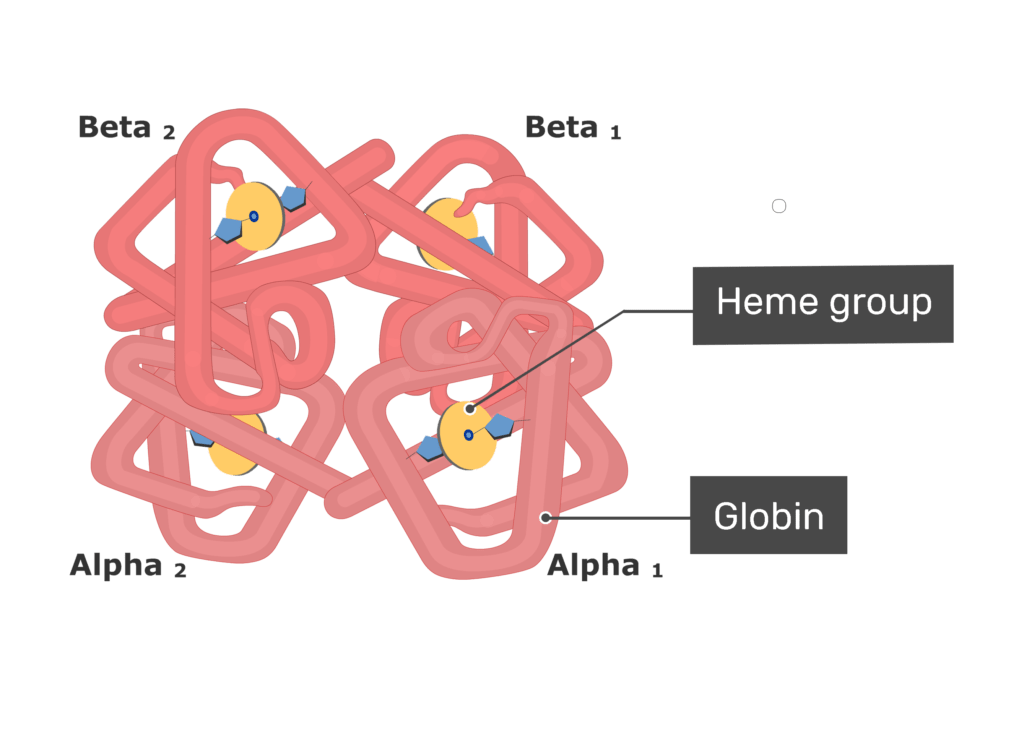
\includegraphics[width=0.8\linewidth]{img/Sheffield, 2017.png}
    \caption{Haemoglobin (Hb) made up of two alpha and two beta globin proteins featuring a iron haem (heme) group (Sheffield, 2017).}
    \label{fig:enter-label}
\end{figure}


Sickle Cell Disease (SCD) is an autosomal recessive disorder where an abnormal gene is inherited from both parents, leading to SCD. If only one copy is inherited, they can become carriers called sickle cell trait (HbAS), where they do not typically express the gene, but due to the dominant expression of the gene, individuals with HbAS only express sickle-shaped RBCs when blood is deoxygenated (Rees and Gibson, 2011).
SCD was first recorded in 1910 by James Herrick, a cardiologist in Chicago when treating a black patient with respiratory problems, he had noted the ‘peculiar elongated
and sickle-shaped’ blood cells when examining them under a microscope, his patient, Walter Clement Noel, shortly died of pneumonia (Schnog et al., 2004) (Steensma, Kyle, and Shampo, 2010).

\begin{figure}
    \centering
    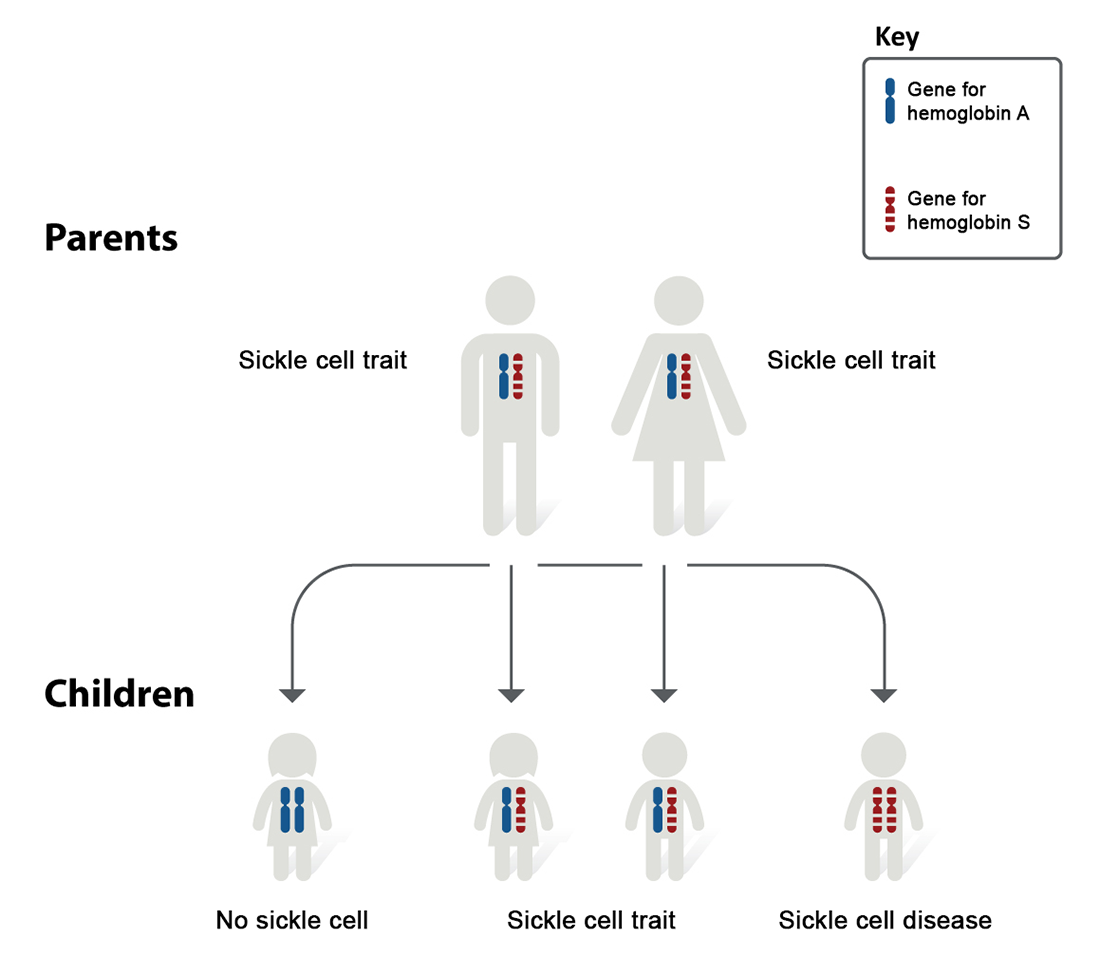
\includegraphics[width=0.5\linewidth]{img/National Heart, Lung and Blood Institute, 2022.png}
    \caption{Sickle Cell Disease inheritance pattern (National Heart, Lung and Blood Institute, 2022)}
    \label{fig:enter-label}
\end{figure}

SCD is characterised by a mutation of the HBB gene, which provides the protein for beta-globin, a crucial protein for haemoglobin function. In SCD, the HBB gene undergoes a point missense mutation where an adenine (A) nucleotide is substituted for a thymine (T) in the sixth codon region in the beta-globin gene; this is characterised by its ‘GTG’ codon pair, coding for glutamic acid, to ‘GAG,’ coding for valine; this leads to the formation of haemoglobin S (HbS) instead of a normal haemoglobin A (HbA) (Kato et al., 2018). Due to valine having hydrophobic (water-opposing) properties when compared to its normal protein glutamic acid, which is hydrophilic (water-attracting), this leads to the polymerisation of the haemoglobin structure when oxygen saturation is low; this in turn causes the haemoglobin to show its characteristic sickle cell shape. Sickle cells are more prone to clump together, causing blockages in the bloodstream; these blockages cause vaso-occlusive crisis (VOC), a painful condition affecting the tissue. (Serjeant, 1997) (Kato et al., 2018). 

\subsection{Risk Factors}
The severity of SCD is affected by two main genetic factors: firstly, the concentration of fetal haemoglobin (HbF). The continued high concentration of HbF in individuals with SCD has been seen to reduce the negative effects of SCD, such as increasing life expectancy and reducing acute episodes of pain (Platt et al., 1991).
Additionally, the co-inheritance of alpha-thalassemia trait, a condition that is defined by the deletion of a-globin chains within the haemoglobin (Farashi and Harteveld, 2018), was found in 30\% of African patients with sickle cell (Higgs et al., 1982) and at rates of 50\% in Saudi and Indian patients (M. Andrew Padmos et al., 1991). A-thalassemia makes it so the haemoglobin concentration is reduced in red blood cells, thus reducing the frequency of HbS polymerisation; this allows haemoglobin concentrations to increase while also decreasing the rate of haemolysis (cell degradation), However if no a-globin genes are inherited (due to mutation or genetic disease) the RBC cannot hold enough oxygen for bodily function, leading to premature death. . It's seen that this can increase the frequency of vaso-occlusive crises (VOC), a painful condition caused by sickle cells clumping and blocking blood to tissues, due to the increase in blood viscosity (Rees and Gibson, 2011).

\begin{figure}
    \centering
    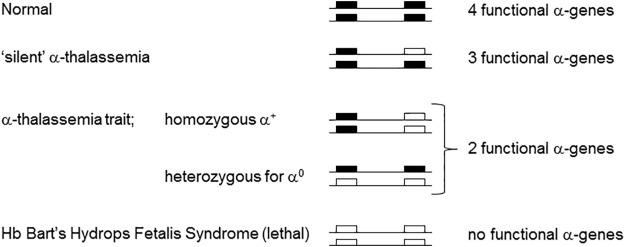
\includegraphics[width=0.8\linewidth]{img/Farashi and Harteveld, 2018, Figure 2.jpg}
    \caption{a-thalassemia types based on functional a-genes. (Farashi and Harteveld, 2018, Figure 2)}
    \label{fig:enter-label}
\end{figure}

Environmental factors such as cold or windy weather have been linked to acute VOC in patients (Jones et al., 2005), and in Jamaica, a tropical country, acute VOC hospitalisation rates were seen to increase after the occurrence of rain (Redwood et al., 1976). Importantly, malaria presence is shown to increase the risk of death of individuals with SCD, as haemoglobin rates are already impacted, causing severe anaemia than those with normal haemoglobin (Rees and Gibson, 2011).

\subsection{Health and Quality of Life}
Health has been shown to be impacted on individuals with SCD, especially those in underdeveloped communities. Haemolytic anaemia is present in nearly all SCD cases, but its effects are lessened in individuals with full alpha and beta thalassemia pairs or a high HbF\% (Schnog et al., 2004). SCD causes individuals red blood cells to have a significantly reduced lifespan of 17-20 days when compared to a healthy lifespan of 120 days, and inorder for the body to compensate for this reduced oxygen-carrying capacity, individuals develop hyperdynamic circulation, where the heart pumps more blood than usual, but due to the dilation of blood vessels, it leads to an overall decrease in blood pressure, putting them at risk of hypertension (Schnog et al., 2004) (Nath, Katusic, and Gladwin, 2004).
Another detriment to health is vaso-occlusive crisis (VOC). This is a condition where sickled cells clump up and form blockages in the microcirculation network (arterioles, capillaries, and venules) (Bentov and Reed, 2015). Occlusion in the bone marrow leads to ischemia (reduction of blood supply), which is observed with excruciating pain in the spine, femura, ribs, and sternum; such cases often lead to hospitalisation, where it is treated with opioids such as morphine and lidocaine (Schnog et al., 2004).
It is estimated that individuals with SCD live 22 fewer years than people without SCD (54 vs 76 years) (Lubeck et al., 2019). In combination with lower life expectancy, quality of life is also lowered for individuals due to medication dependence; typically, opioids such as morphine and oxycodone are used to manage pain from VOC, but due to the nature of such drugs, addiction is commonplace with individuals, leading to a dependence on drugs for treatment of VOC (Brandow et al., 2020) (Geller and O’Connor, 2008).

\section{Epidemiology}
\subsection{Incidence, Prevalence, and Mortality}
The incidence (rate of new cases for a population over a specified time (Tenny and Boktor, 2023)) of SCD in 2021 was over half a million, with more than 80\% of cases occurring in sub-Saharan Africa (Thomson, 2023), and the prevalence (number of people living with a characteristic in a specified time (National Institute of Mental Health, 2020)) of SCD being 8 million globally (Thomson, 2023).

\begin{figure}
    \centering
    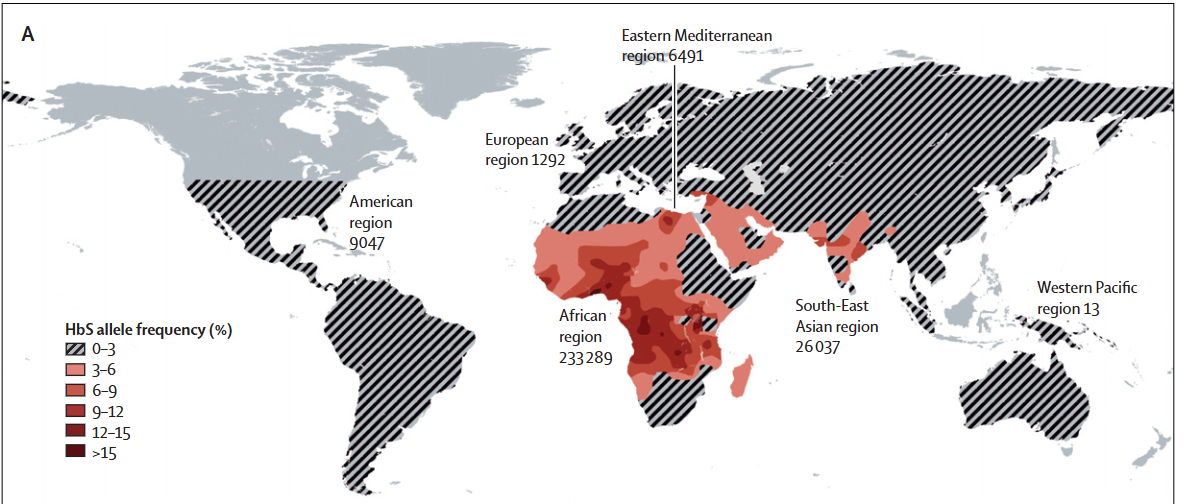
\includegraphics[width=0.8\linewidth]{img/Rees, Williams and Gladwin, 2010, Figure 3.png}
    \caption{ This map shows the distribution of the HbS allele. (Rees, Williams and Gladwin, 2010, Figure 3)}
    \label{fig:enter-label}
\end{figure}


The mortality rate (rate of death for a certain group of people over a period of time (National Institute of Health, 2019)) for <5 years was 60\% on average in African countries when compared to western countries at a <5\% mortality rate. Where the main causes of death were pneumonia, malaria, and acute anaemia (Thomson, 2023).

\begin{figure}
    \centering
    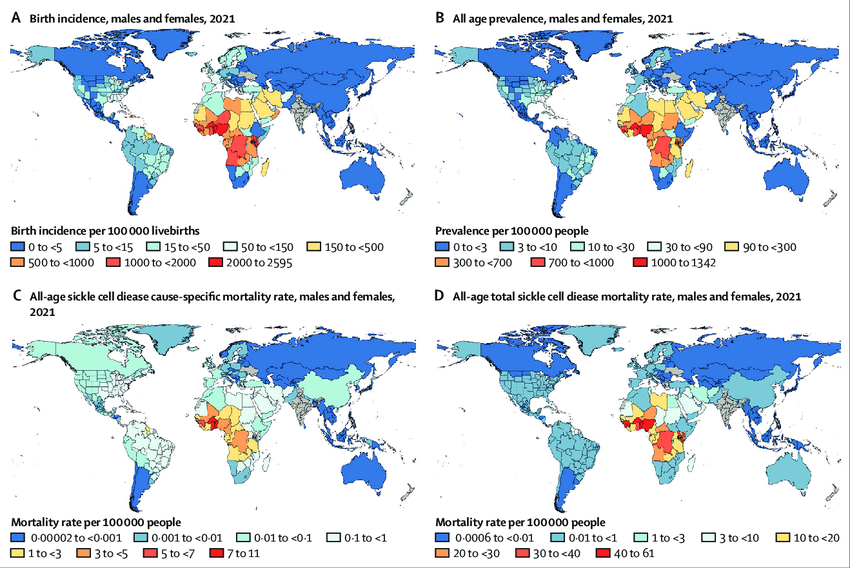
\includegraphics[width=0.8\linewidth]{img/Thomson, 2023, Figure 3.png}
    \caption{Maps of total sickle cell disease rates per 100 000 population. (Thomson, 2023, Figure 3)}
    \label{fig:enter-label}
\end{figure}

\begin{table}[]
    \begin{center}
        \begin{tabular}{llll}
         & Patients & Deaths & Mortality Rate \% \\
        Children (\textless{}18 years old) & 420 & 44 & 10.48 \\
        Adults (\textgreater{}18 years old) & 1256 & 237 & 18.87 \\
        All patients & 1676 & 281 & 16.77
        \end{tabular}
    \end{center}
    \caption{Mortality Rate of Individual with SCD within Rio de Janeiro, Brazil. (Lobo et al., 2018, Table 2)}
    \label{tab:my-table}
\end{table}

\subsection{Irregularites of Data}
Though all statistics may not be reliable due to the economic disproportion, especially in Africa, where diagnostic facilities may be poor and the practice of routine screening is not performed, unlike in developed countries, where SCD is tested in all newborns (Rees, Williams, and Gladwin, 2010).
Another reason for the higher SCD rates in African countries is the protection from malaria, where individuals who have this characteristic passed it down, due to malaria selection, which resulted in higher frequencies in regions prone to malaria (Rees, Williams, and Gladwin, 2010).  



\section{Prevention}
SCD is most commonly diagnosed at newborn screening using methods such as protein
electrophoresis or chromatography (A. Denomme et al., 2009) (Rees, Williams, and Gladwin, 2010).

\subsection{CRISPR-Cas9 Technology}
CRISPR-Cas9 technologies, such as Casgevy, are used to fix the root cause of SCD, the faulty beta-globin gene. This technology is used to edit blood stem cells on the BCL11A gene, which produces HbF. In this, it increases the production of HbF, which is less susceptible to sickling to reduce the frequency of VOC. Treatment for Casgevy occurs in individuals 12 years or older (Adashi, Gruppuso, and Cohen, 2024).
\subsection{IVF Genetic Testing}
If individuals choose to prevent SCD before birth, in vitro fertilisation (IVF) technologies such as preimplantation genetic testing (PGT) can be used to ensure this (Speer, 2019). In this, trophectoderm cells are collected in vitro and are analysed for the mutated trait; this is done for both the sperm and egg. After analysis, the egg is fertilised in vitro and reintroduced to the uterus (Combs et al., 2023). 

\section{Treatment}
Patients struggling with SCD VOC are given analgesics such as opioids to manage pain; additionally, they are given vitamins that include folic acid to promote RBC production, and saline is used to give fluids to increase blood viscosity, reducing the risk of further VOC (A. Denomme et al., 2009).
Another method of treatment is hydroxyurea (HU) or hydroxycarbamide, a cytotoxic drug given to increase HbF concentrations and increase overall Hb concentrations. HU additionally lowers platelet count but at the cost of lowering white blood cell count (A. Denomme et al., 2009) (Rees, Williams, and Gladwin, 2010).

\subsection{Research for SCD}
CRISPR-Cas9 technologies are being used to research gene therapies for SCD; currently, lovotibeglogene autotemcel (Lyfgenia) is being researched and was recently FDA approved for SCD. Using modified beta-globin genes in the patients stem cells, this treatment produces a haemoglobin less prone to sickling (Kanter et al., 2024) (American Society of Hematology, 2024).
Another research programme being studied by the American Society of Hematology are novel drugs, to develop inhibitors that target the polymerisation inducers in HbS, they hope to use pyruvate kinase activators to address the chronic pain and organ damage from VOC (American Society of Hematology, 2024).

\begin{thebibliography}{99}

\bibitem{gilchrist_2019_mutation}Gilchrist, D. Mutation. (National Human Genome Research Institute,2019), \url{https://www.genome.gov/genetics-glossary/Mutation}
\bibitem{schrader_2003_mutagens}Schrader, T. MUTAGENS. {\em Encyclopedia Of Food Sciences And Nutrition}. \textbf{2} pp. 4059-4067 (2003)
\bibitem{chidrawi_2018_biology}Chidrawi, G., Robson, M., Bradstock, S. \& Thrum, E. Biology in focus. Year 12. (Cengage Learning Australia,2018,10)
\bibitem{kato_2018_sickle}Kato, G., Piel, F., Reid, C., Gaston, M., Ohene-Frempong, K., Krishnamurti, L., Smith, W., Panepinto, J., Weatherall, D., Costa, F. \& Vichinsky, E. Sickle Cell Disease. {\em Nature Reviews Disease Primers}. \textbf{4} (2018,3), \url{https://www.nature.com/articles/nrdp201810}
\bibitem{serjeant_1997_sicklecell}Serjeant, G. Sickle-cell disease. {\em The Lancet}. \textbf{350} pp. 725-730 (1997,9)
\bibitem{shendure_2015_the}Shendure, J. \& Akey, J. The origins, determinants, and consequences of human mutations. {\em Science}. \textbf{349} pp. 1478-1483 (2015,9)
\bibitem{platt_1991_pain}Platt, O., Thorington, B., Brambilla, D., Milner, P., Rosse, W., Vichinsky, E. \& Kinney, T. Pain in Sickle Cell Disease. {\em New England Journal Of Medicine}. \textbf{325} pp. 11-16 (1991,7)
\bibitem{rees_2011_biomarkers}Rees, D. \& Gibson, J. Biomarkers in sickle cell disease. {\em British Journal Of Haematology}. \textbf{156} pp. 433-445 (2011,11)
\bibitem{farashi_2018_molecular}Farashi, S. \& Harteveld, C. Molecular basis of a-thalassemia. {\em Blood Cells, Molecules, And Diseases}. \textbf{70} pp. 43-53 (2018,5), \url{https://www.sciencedirect.com/science/article/pii/S1079979617301493}
\bibitem{higgs_1982_the}Higgs, D., Aldridge, B., Lamb, J., Clegg, J., Weatherall, D., Hayes, R., Grandison, Y., Lowrie, Y., Mason, K., Serjeant, B. \& Serjeant, G. The Interaction of Alpha-Thalassemia and Homozygous Sickle-Cell Disease. {\em New England Journal Of Medicine}. \textbf{306} pp. 1441-1446 (1982,6)
\bibitem{mandrewpadmos_1991_two}Padmos, M., Roberts, G., Sackey, K., Kulozik, A., Bail, S., Morris, J., Serjeant, B. \& Serjeant, G. Two different forms of homozygous sickle cell disease occur in Saudi Arabia.  (1991,9)
\bibitem{jones_2005_windy}Jones, S., Duncan, E., Thomas, N., Walters, J., Dick, M., Height, S., Stephens, A., Thein, S. \& Rees, D. Windy weather and low humidity are associated with an increased number of hospital admissions for acute pain and sickle cell disease in an urban environment with a maritime temperate climate. {\em British Journal Of Haematology}. \textbf{131} pp. 530-533 (2005,11)
\bibitem{redwood_1976_climate}Redwood, A., Williams, E., Desal, P. \& Serjeant, G. Climate and painful crisis of sickle-cell disease in Jamaica.. {\em BMJ}. \textbf{1} pp. 66-68 (1976,1)
\bibitem{nath_2004_the}Nath, K., Katusic, Z. \& Gladwin, M. The Perfusion Paradox and Vascular Instability in Sickle Cell Disease. {\em Microcirculation}. \textbf{11} pp. 179-193 (2004,1)
\bibitem{bentov_2015_the}Bentov, I. \& Reed, M. The effect of aging on the cutaneous microvasculature. {\em Microvascular Research}. \textbf{100} pp. 25-31 (2015,7), \url{https://www.ncbi.nlm.nih.gov/pmc/articles/PMC4461519/}
\bibitem{LOBO201837}Castro Lobo, C., Nascimento, E., Jesus, L., Freitas, T., Lugon, J. \& Ballas, S. Mortality in children, adolescents and adults with sickle cell anemia in Rio de Janeiro, Brazil. {\em Hematology, Transfusion And Cell Therapy}. \textbf{40}, 37-42 (2018), \url{https://www.sciencedirect.com/science/article/pii/S1516848417301330}
\bibitem{lubeck_2019_estimated}Lubeck, D., Agodoa, I., Bhakta, N., Danese, M., Pappu, K., Howard, R., Gleeson, M., Halperin, M. \& Lanzkron, S. Estimated Life Expectancy and Income of Patients With Sickle Cell Disease Compared With Those Without Sickle Cell Disease. {\em JAMA Network Open}. \textbf{2} pp. e1915374 (2019,11), \url{https://www.ncbi.nlm.nih.gov/pmc/articles/PMC6902797/}
\bibitem{brandow_2020_american}Brandow, A., Carroll, C., Creary, S., Edwards-Elliott, R., Glassberg, J., Hurley, R., Kutlar, A., Seisa, M., Stinson, J., Strouse, J., Yusuf, F., Zempsky, W. \& Lang, E. American Society of Hematology 2020 guidelines for sickle cell disease: management of acute and chronic pain. {\em Blood Advances}. \textbf{4} pp. 2656-2701 (2020,6)
\bibitem{geller_2008_the}Geller, A. \& O'Connor, M. The Sickle Cell Crisis: A Dilemma in Pain Relief. {\em Mayo Clinic Proceedings}. \textbf{83} pp. 320-323 (2008,3), \url{https://www.mayoclinicproceedings.org/article/S0025-6196(11)60865-3/fulltext}
\bibitem{sheffield_2017_hemoglobin}Sheffield, S. Hemoglobin - Structure, Function and Diagram | GetBodySmart. (GetBodySmart,2017,5), \url{https://www.getbodysmart.com/respiratory-gases-and-their-transport/hemoglobin-structure/}
\bibitem{nationalheartlungandbloodinstitute_2022_sickle}National Heart, L. \& Institute, B. Sickle Cell Disease - Causes and Risk Factors. (www.nhlbi.nih.gov,2022), \url{https://www.nhlbi.nih.gov/health/sickle-cell-disease/causes}
\bibitem{steensma_2010_walter}Steensma, D., Kyle, R. \& Shampo, M. Walter Clement Noel—First Patient Described With Sickle Cell Disease. {\em Mayo Clinic Proceedings}. \textbf{85} pp. e74-e75 (2010,10), \url{https://www.ncbi.nlm.nih.gov/pmc/articles/PMC2947974/}
\bibitem{medlineplus_paroxysmal}Plus, M. Paroxysmal nocturnal hemoglobinuria: MedlinePlus Genetics. (medlineplus.gov), \url{https://medlineplus.gov/genetics/condition/paroxysmal-nocturnal-hemoglobinuria/}
\bibitem{nationalcancerinstitute_2012}Institute, N. (www.cancer.gov,2012,7), \url{https://www.cancer.gov/publications/dictionaries/genetics-dictionary/def/germline-mutation}
\bibitem{akhtar_2023_down}Akhtar, F. \& Bokhari, S. Down syndrome. (StatPearls Publishing,2023,8), \url{https://www.ncbi.nlm.nih.gov/books/NBK526016/}
\bibitem{nationalheartlungandbloodinstitute_2024_sickle}National Heart \& Institute, B. Sickle Cell Disease - What is Sickle Cell Disease?. (NIH,2024,9), \url{https://www.nhlbi.nih.gov/health/sickle-cell-disease}
\bibitem{richardboland_2017_noncoding}Richard Boland, C. Non-coding RNA: It’s Not Junk. {\em Digestive Diseases And Sciences}. \textbf{62} pp. 1107-1109 (2017,3)
\bibitem{mattick_2022_the}Mattick, J. \& Amaral, P. The Human Genome. (CRC Press,2022,9), \url{https://www.ncbi.nlm.nih.gov/books/NBK595930/}
\bibitem{needs_2023_beta}Needs, T., Gonzalez-Mosquera, L. \& Lynch, D. Beta Thalassemia. (StatPearls Publishing,2023,5), \url{https://www.ncbi.nlm.nih.gov/books/NBK531481/}
\bibitem{majerus_2003_mammalian}Majerus, M. \& Mundy, N. Mammalian melanism: natural selection in black and white. {\em Trends In Genetics}. \textbf{19} pp. 585-588 (2003,11)
\bibitem{hoelzel_2024_genomics}Hoelzel, A., Gkafas, G., Kang, H., Sarigol, F., Le Boeuf, B., Costa, D., Beltran, R., Reiter, J., Robinson, P., McInerney, N., Seim, I., Sun, S., Fan, G. \& Li, S. Genomics of post-bottleneck recovery in the northern elephant seal. {\em Nature Ecology \& Evolution}. \textbf{8} pp. 1-9 (2024,2), \url{https://www.nature.com/articles/s41559-024-02337-4#:~:text=The\%20northern\%20elephant\%20seal\%20was}
\bibitem{tenny_2023_incidence}Tenny, S. \& Boktor, S. Incidence. (StatPearls Publishing,2023,4), \url{https://www.ncbi.nlm.nih.gov/books/NBK430746/}
\bibitem{nationalinstituteofmentalhealth_2020_what}Mental Health, N. What is Prevalence?. (National Institute of Mental Health,2020), \url{https://www.nimh.nih.gov/health/statistics/what-is-prevalence}
\bibitem{thomson_2023_global}Thomson, A. Global, regional, and national prevalence and mortality burden of sickle cell disease, 2000–2021: a systematic analysis from the Global Burden of Disease Study 2021. {\em The Lancet Haematology}. \textbf{10} (2023,6), \url{https://www.sciencedirect.com/science/article/pii/S2352302623001187#:~:text=Sickle\%20cell\%20disease\%20has\%20a,with\%20sickle\%20cell\%20disease\%20globally.}
\bibitem{rees_2010_sicklecell}Rees, D., Williams, T. \& Gladwin, M. Sickle-cell Disease. {\em The Lancet}. \textbf{376} pp. 2018-2031 (2010,12)
\bibitem{nationalinstituteofhealth_2019_nci}Health, N. NCI Dictionary of Cancer Terms. (Cancer.gov,2019), \url{https://www.cancer.gov/publications/dictionaries/cancer-terms/def/mortality}
\bibitem{adenomme_2009_consortium}A. Denomme, G., Westhoff, C., Castilho, L. \& Reid, M. Consortium for Blood Group Genes (CBGG): 2008 report. {\em Immunohematology}. \textbf{25} pp. 75-78 (2009,1)
\bibitem{kanter_2024_lovotibeglogene}Kanter, J., Chawla, A., Thompson, A., Kwiatkowski, J., Parikh, S., Mapara, M., Rifkin-Zenenberg, S., Aygun, B., Kasow, K., Gupta, A., Zhang, L., Sheldon-Waniga, E., Gallagher, M., Gruppioni, K., Elliot, H., Pierciey, F., Walters, M. \& Tisdale, J. Lovotibeglogene Autotemcel Gene Therapy for Sickle Cell Disease: 60 Months Follow-up. {\em Journal Of Sickle Cell Disease}. \textbf{1} (2024,6), \url{https://academic.oup.com/jscd/article/1/Supplement_1/yoae002.002/7686711?login=false}
\bibitem{americansocietyofhematology_2024_ash}Hematology, A. ASH SICKLE CELL DISEASE RESEARCH PRIORITIES.  (2024), \url{https://www.hematology.org/-/media/hematology/files/research/scd-research-priorities_2024-update_18sept24_final.pdf}
\bibitem{adashi_2024_crispr}Adashi, E., Gruppuso, P. \& Cohen, I. CRISPR Therapy of Sickle Cell Disease: The Dawning of the Gene Editing Era. {\em The American Journal Of Medicine}. \textbf{137} (2024,1), \url{https://www.sciencedirect.com/science/article/pii/S0002934323007982?via\%253Dihub}
\bibitem{combs_2023_preimplantation}Combs, J., Dougherty, M., Yamasaki, M., DeCherney, A., Devine, K., Hill, M., Rothwell, E., O’Brien, J. \& Nelson, R. Preimplantation genetic testing for sickle cell disease: a cost-effectiveness analysis. {\em F\&S Reports}. \textbf{4} pp. 300-307 (2023,9)
\bibitem{speer_2019_how}Speer, J. How IVF and Genetic Testing Can Help Prevent Sickle Cell Anemia. (www.illumefertility.com,2019,9), \url{https://www.illumefertility.com/fertility-blog/how-ivf-and-genetic-testing-can-prevent-sickle-cell-anemia}

\end{thebibliography}



\end{document}
